% (C) Marc Lijour, 2016-2017 
% Licensed under a Creative Commons License BY-SA
% https://creativecommons.org/licenses/by-sa/2.5/ca/
% Presentation for the Small Business Digitization Initiative (SBDI) training program
% see http://www.ictc-ctic.ca/small-business-digitization-initiative/ 
% authored by Marc Lijour, April 2017 
% for the session running from January 2017 to September 2017
% 
% ======================================================================================================
%                                     Odoo: What is it?
% ======================================================================================================
\section{Odoo: the course ERP}
% --------------------- Short intro --------------------------
\subsection{A Short Introduction to Odoo}
\frame{
	\frametitle{Small Business Digitization Initiative}
	\framesubtitle{Odoo -- The course ``ERP''}

	\begin{figure}
	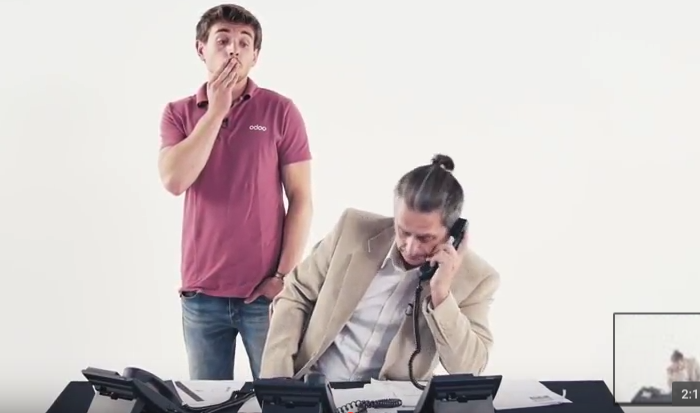
\includegraphics[width=11.5cm]{../pics/odoo-youtube-notERP}
	\caption{\tiny\url{https://www.youtube.com/watch?v=2dhyhamLm6M&list=PL1-aSABtP6AALA_4hW2TyYIioOVEGQ3yf&index=6}}
	\end{figure}
}

%\frame{
%	\frametitle{}
%	\framesubtitle{}
%}

\frame{
	\frametitle{A Short Introduction to Odoo}
	\framesubtitle{Odoo in a few words}
	\begin{figure}	
		\centering
		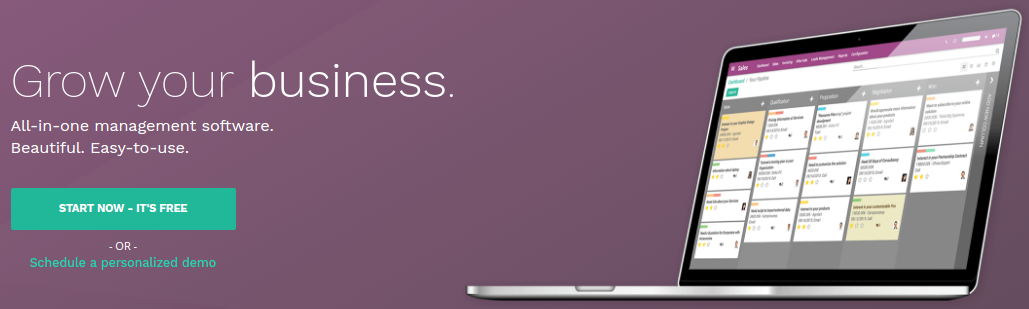
\includegraphics[width=12cm]{../pics/odoo-tagline}
		\caption{\url{https://www.odoo.com} (\cite{odoosa})}
	\end{figure}
}

\frame{
	\frametitle{A Short Introduction to Odoo}
	\framesubtitle{Value Proposition}
	\begin{figure}	
		\centering
		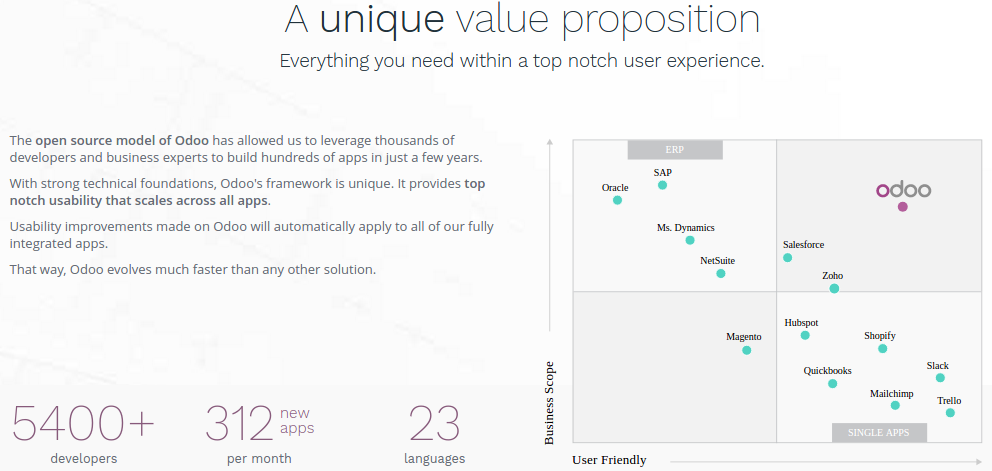
\includegraphics[width=12cm]{../pics/odoo-unique-value-prop}
	\end{figure}
}

\frame{
	\frametitle{A Short Introduction to Odoo}
	\framesubtitle{Creating Apps is easy (no technical background required)}
	\begin{figure}	
		\centering
		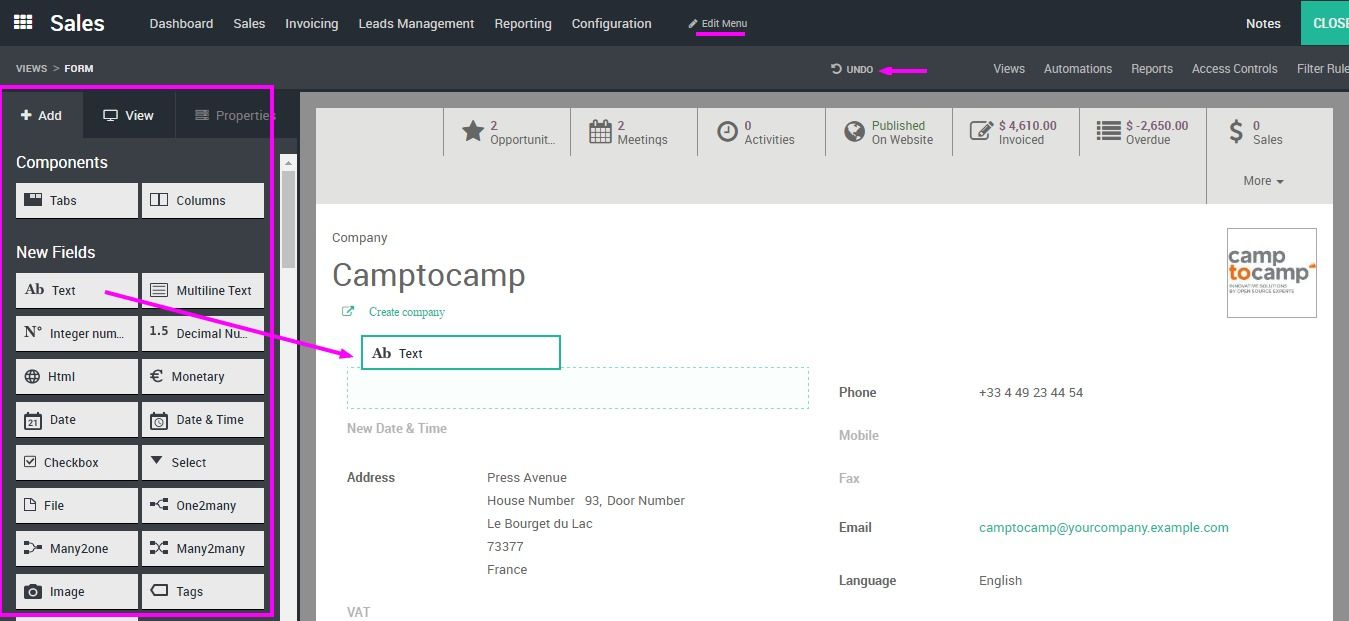
\includegraphics[width=12cm]{../pics/odoo-studio-saas14}
		\caption{\href{https://www.youtube.com/watch?v=xCvFZrrQq7k}{Odoo ``Studio''} is available on the Enterprise and Online versions}
	\end{figure}
}

\frame{
	\frametitle{A Short Introduction to Odoo}
	\framesubtitle{\emph{Great User Experience Award} and the \emph{2017 Rising Star}}
	\begin{figure}	
		\centering
		
\includegraphics[width=12cm]{../pics/odoo-awards2017}
		\caption{\href{https://www.odoo.com/blog/odoo-news-5/post/odoo-wins-two-prestigious-erp-software-awards-from-financesonline-362}{Odoo News April 2017}}
	\end{figure}
}

% --------------------- Why Odoo in this course --------------------------
\subsection{Why we chose Odoo}
\frame{
	\frametitle{Why we chose Odoo}
	\framesubtitle{In a few words}
	\begin{itemize}
		\item Simple and Easy to use (and to learn)
		\pause
		\item Cheap for students 
			\\{\tiny (Open Source version is always \$0; furthermore SBDI students have access to Odoo Online for free)}
		\pause
		\item Cheap for employers 
			\\{\tiny (Odoo online: one app = \$0 regardless of the number of users; other apps are affordable)}
		\pause
		\item Extensible (Official apps + thousands of open source apps)
		\pause
		\item Beautiful
		\pause
		\item Odoo Community in Toronto and Montreal
	\end{itemize}
}

\frame{
	\frametitle{Why we chose Odoo}
	\framesubtitle{10,000 Apps available}
	\begin{itemize}[<+->]
		\item 10,000 integrated apps only after 2 years the Appstore exists
		\item 12 new apps released every day
		\item Every month, 80,000 apps are downloaded by Odoo users
		\item 86\% of the apps are open source! 
		\item Read the \href{https://www.odoo.com/blog/odoo-news-5/post/10000-apps-in-the-odoo-app-store-352}{Announcement}
	\end{itemize}
}

\frame{
	\frametitle{Why we chose Odoo}
	\framesubtitle{Odoo Communication Association (OCA)}
	\begin{figure}	
		\centering
		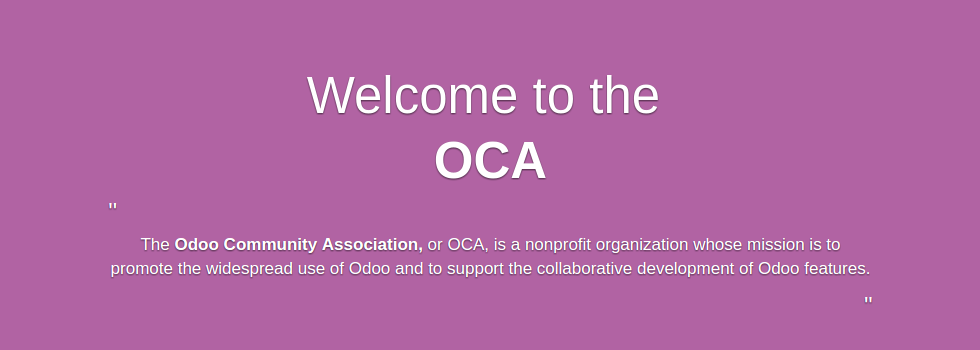
\includegraphics[width=12cm]{../pics/odoo-OCA}
		\caption{\url{https://odoo-community.org} (\cite{oca})}
	\end{figure}
}


\frame{
	\frametitle{Why we chose Odoo}
	\framesubtitle{Odoo Communication Association (OCA) Apps}
	\begin{figure}	
		\centering
		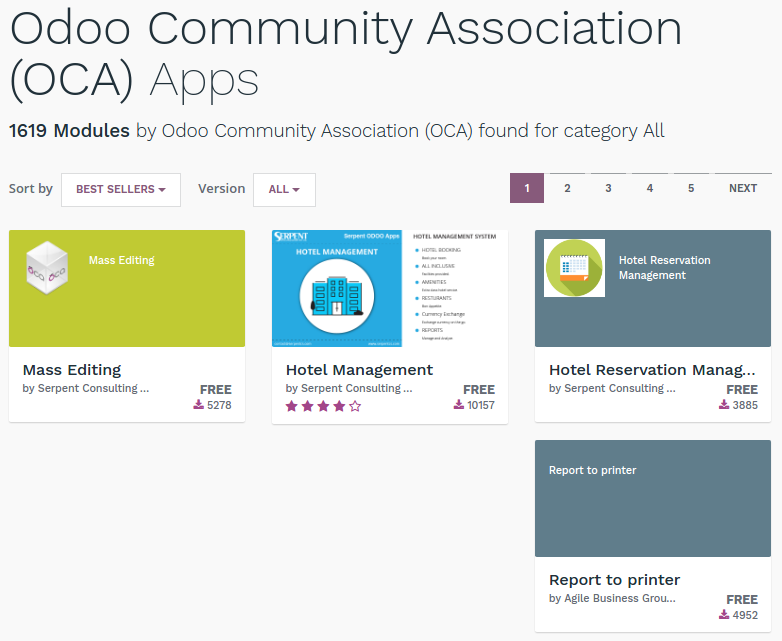
\includegraphics[height=6cm]{../pics/odoo-OCA-apps}
		\caption{See the \href{https://www.odoo.com/apps/modules?author=Odoo\%20Community\%20Association\%20(OCA)}{OCA section on Odoo.com} and \url{https://github.com/OCA} (\cite{ocagithub,ocaappsonodoo})}
	\end{figure}
}


\frame{
	\frametitle{Why we chose Odoo}
	\framesubtitle{Thousands of Open Source modules}
	\begin{figure}	
		\centering
		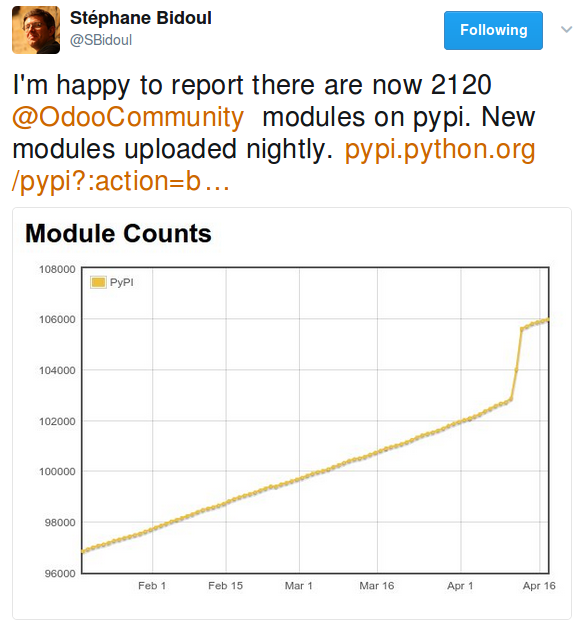
\includegraphics[height=6cm]{../pics/odoo-pypi}
	\end{figure}
}


% --------------------- Version of Odoo --------------------------
\section{Versions of Odoo}
\frame{
	\frametitle{Versions of Odoo}
	\framesubtitle{Opencore Model}
	\begin{itemize}[<+->]
		\item Odoo Community
			\\{\tiny$\surd$ Open Source, Free, Forever}
		\item Odoo Enterprise
			\\{\tiny$\surd$ added-value Enterprise Modules, run by the Odoo customer, better choice for large and complex deployments}
		\item Odoo Online (aka SaaS)
			\\{\tiny$\surd$ added-value Enterprise Modules, run by Odoo SA, free support, low TCO, less flexibility $\rightarrow$ course databases (2)}
		\item Developer version (see Tech Labs)
		\item See \url{https://www.odoo.com/pricing} 
			\\and \url{https://www.odoo.com/page/editions} for more details
	\end{itemize}
}

\frame{
	\frametitle{Why we chose Odoo}
	\framesubtitle{Odoo Versions}
	\begin{figure}	
		\centering
		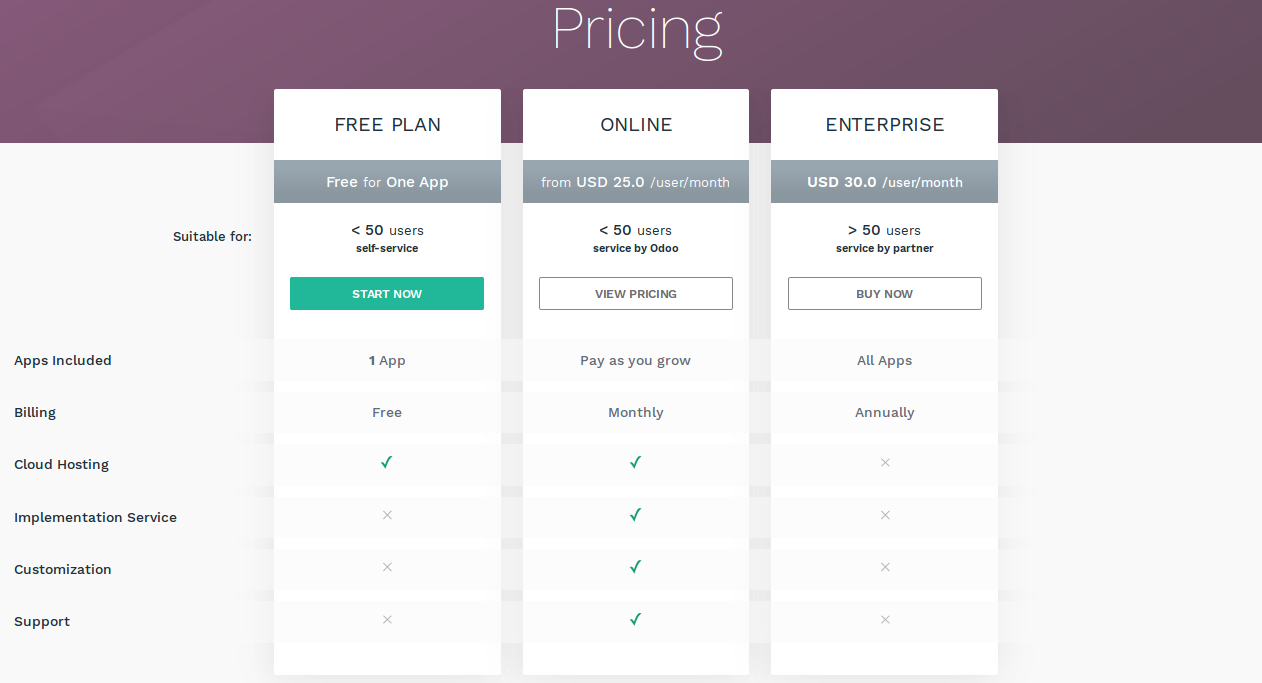
\includegraphics[height=6cm]{../pics/odoo-pricing}
	\end{figure}
}

\frame{
	\frametitle{Try different versions of Odoo}
	\begin{figure}
		\centering
		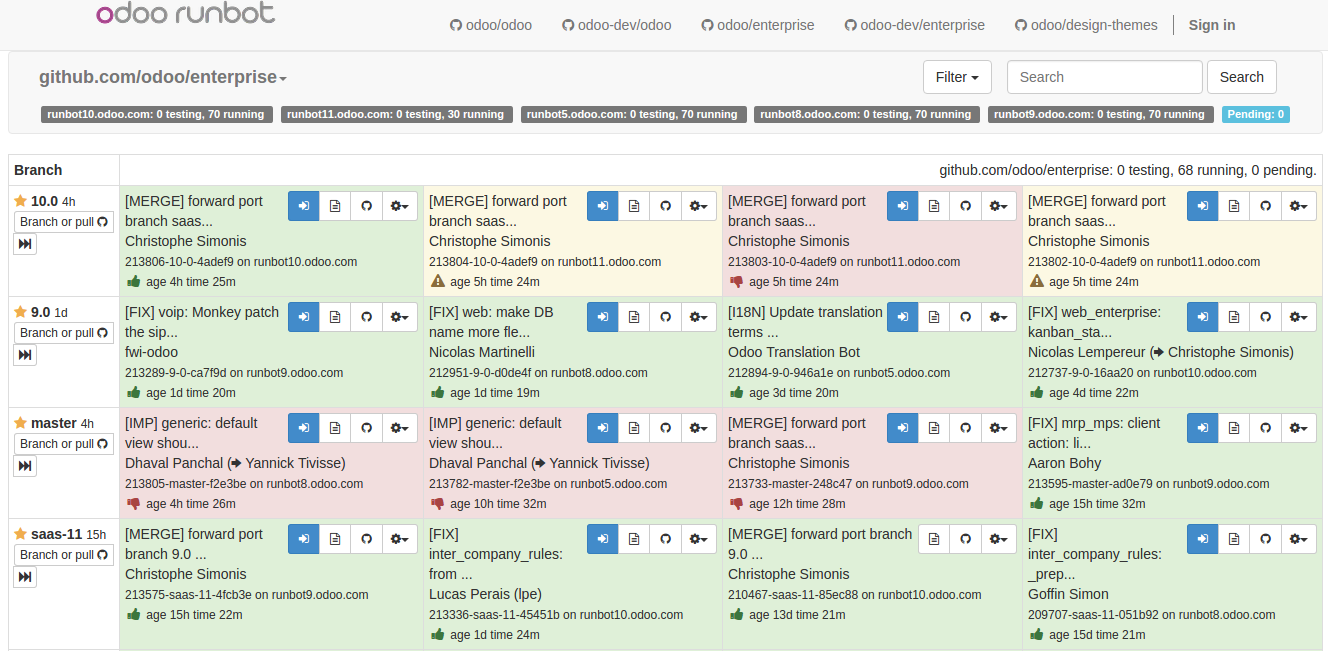
\includegraphics[width=12cm]{../pics/odoo-runbot}
		\caption{\url{http://runbot.odoo.com/runbot}}
	\end{figure}
}

\frame{
	\frametitle{The future of Odoo}
	\begin{figure}
		\centering
		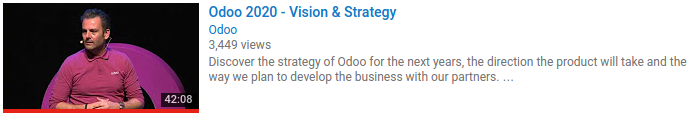
\includegraphics[width=12cm]{../pics/odoo-vision2020}
		\caption{\url{https://www.youtube.com/watch?v=v8eumtr3X1Q}}
	\end{figure}
	\begin{figure}
		\centering
		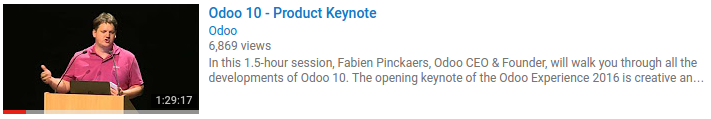
\includegraphics[width=12cm]{../pics/odoo-odoo10keynote}
		\caption{\url{https://www.youtube.com/watch?v=TMno_mDkBRE}}
	\end{figure}
}

% ======================================================================================================
%                                     Additional Odoo Training
% ======================================================================================================
\section{Additional Odoo Training}
\frame{
	\frametitle{Odoo Training}
	\framesubtitle{Pick a career path}
	\begin{itemize}[<+->]
		\item Functional Training
		\item Technical Training
	\end{itemize}
}

\frame{
	\frametitle{Odoo Training}
	\framesubtitle{Courses on Udemy}
	\begin{figure}	
		\centering
		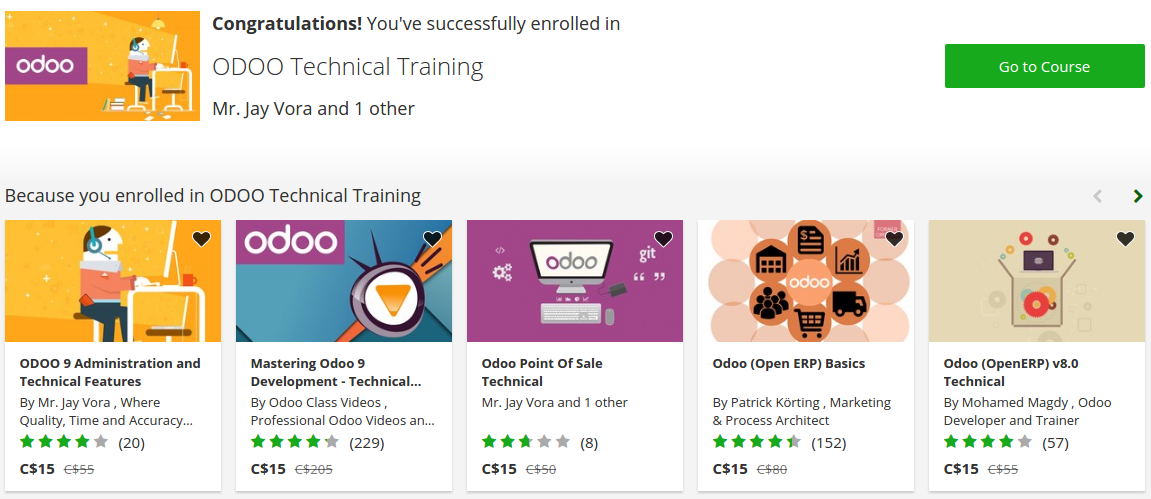
\includegraphics[width=12cm]{../pics/udemy-sample-odoo-courses}
		\caption{\tiny \url{https://www.udemy.com/odoo-technical/}}
	\end{figure}
}

\frame{
	\frametitle{Odoo Training}
	\framesubtitle{Books on O'Reilly Safari (there is plenty)}
	\begin{figure}	
		\centering
		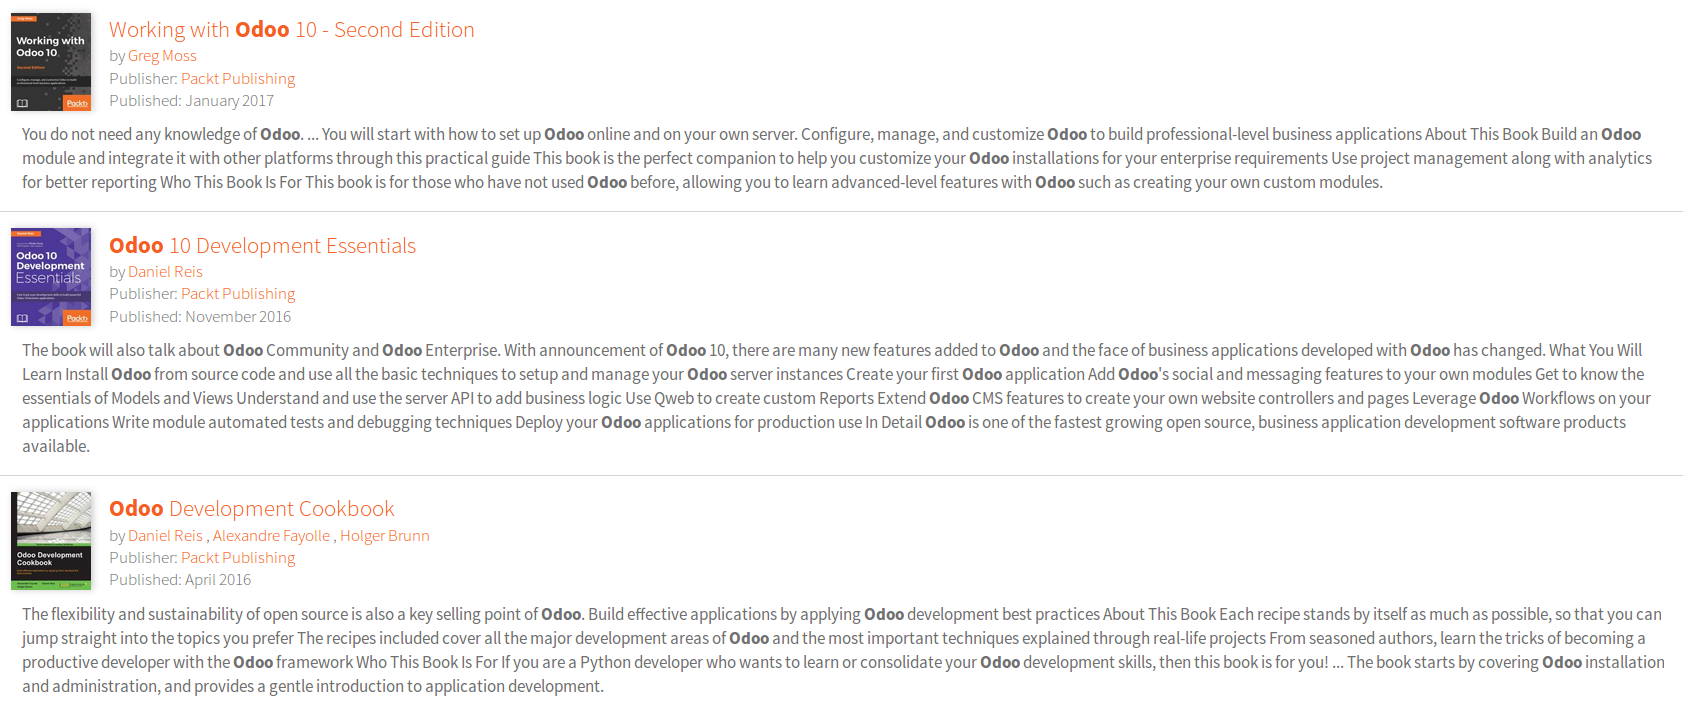
\includegraphics[width=12cm]{../pics/odoo-safari}
		\caption{\href{http://my.safaribooksonline.com/}{O'Reilly Safari} is freely accessible with a Toronto Public Library Card (\cite{oreillysafari})}
	\end{figure}
}

\frame{
	\frametitle{Odoo Training}
	\framesubtitle{from Odoo S.A.}
	\begin{figure}
		\centering
		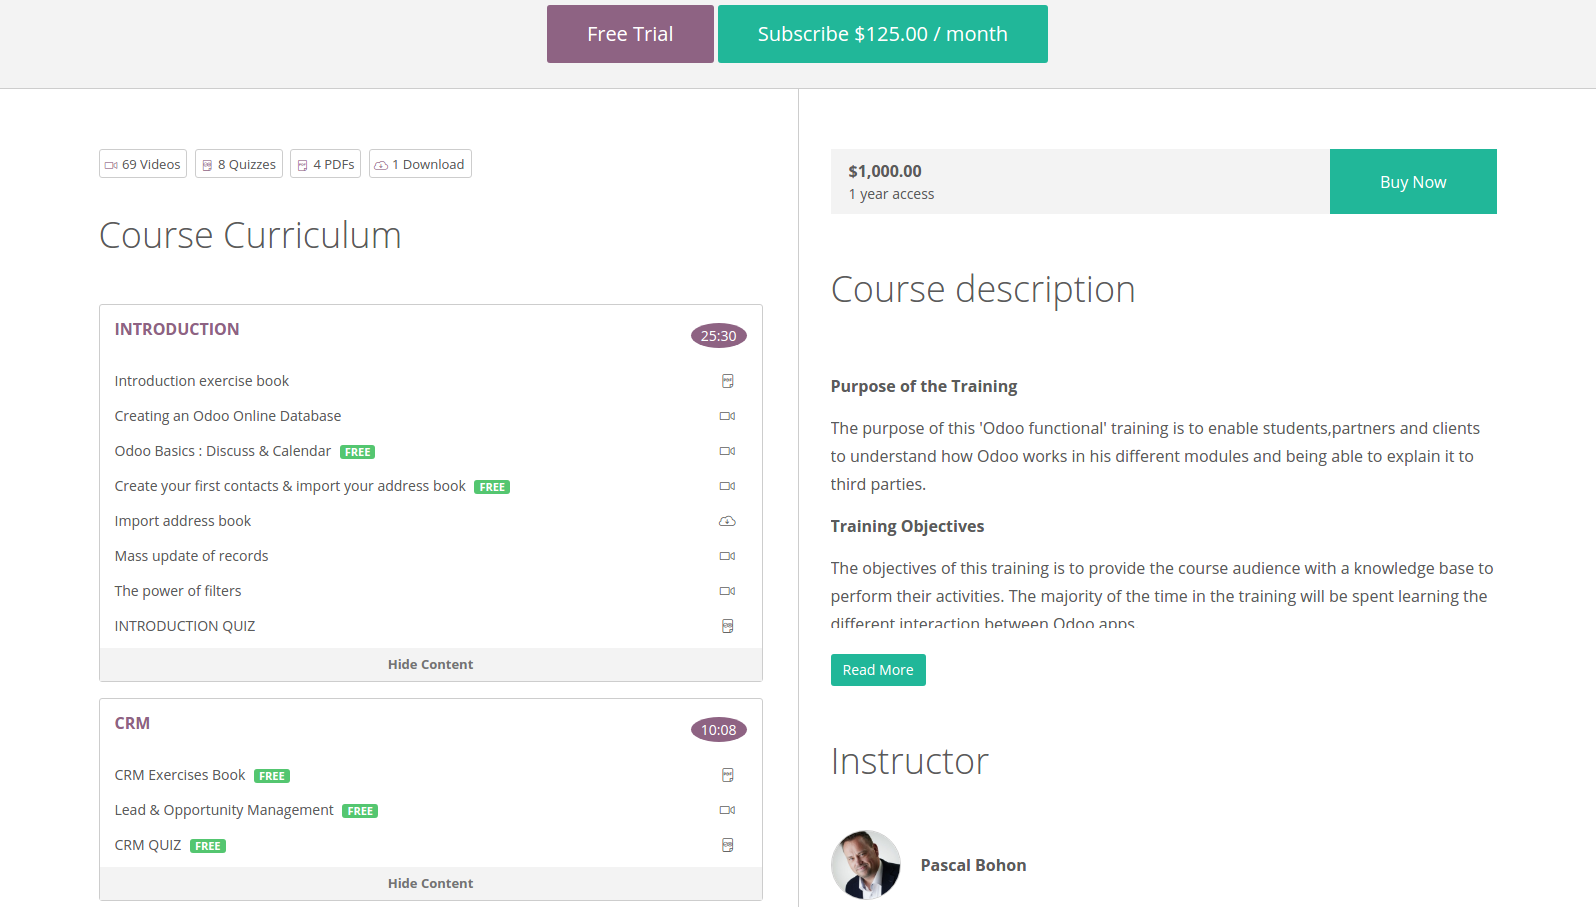
\includegraphics[width=12cm]{../pics/odoosatraining}
		\caption{\href{https://odoo.thinkific.com/courses/odoo-functional}{Free trial (\cite{odoosatraining})}}
	\end{figure}
}

\frame{
	\frametitle{Odoo Training}
	\framesubtitle{ERP Courses on \href{http://edx.org}{edX}}
	\begin{figure}	
		\centering
		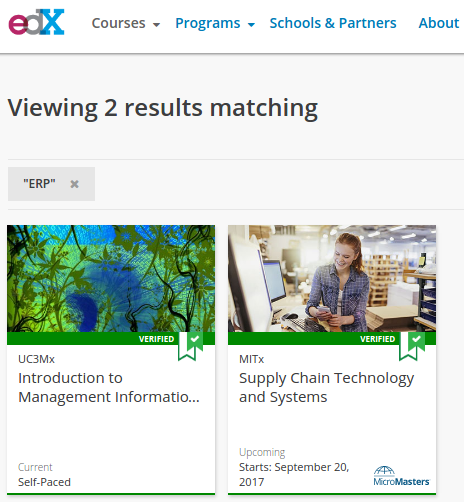
\includegraphics[height=6cm]{../pics/edx-ERP-courses}
		\caption{Top courses available at \href{http://edx.org}{edX}}
	\end{figure}
}

% ~ ~ ~ References
% ======================================================================================================
%                                     References
% ======================================================================================================
\section{References}
\frame[allowframebreaks]{
	\frametitle{Odoo: the course ERP}
	\framesubtitle{References}
	% keyword refers to bib file: references-KEYWORD.bib, and to the Tex file: section-KEYWORD.tex
	\printbibliography[keyword=odoo-course-erp]
}


